


\section{Setting up the environment}

The development process of DroidGuardian comprised several stages that corresponding to the layer level that was being handled. The kernel module requested a completely different environment when compared to the Java layer implementation environment.

In order to fully understand the \gls{lsm} framework it was necessary to manipulate a real Linux kernel, as well as compile and install. Since the work machine used was a \textit{MacBook Pro}, a new partition was created to install the \textit{Xubuntu}. This is a different flavor of \textit{Ubuntu Linux} operating system that provides a light user interface. Basically, the only used program was the console, because all required steps could be executed through the command line and using \textit{Vim}. This is why a lighter and simpler user interface was enough to carry on the desired tasks on the Linux environment. The new partition was created using \textit{rEFIt}\footnote{http://refit.sourceforge.net}.

Running Linux on a new partition provided speed and efficiency when setting up the Android environment, to build and launch a new image on the emulator. However, handling loadable kernel modules on a separated partition proved to be a mistake, due to the system's blocking when kernel failures were reached by programming errors. To overcome this inconvenience, programming tests with loadable kernel modules started to be done in a virtual machine. This way, if the code contained flaws that could led to a kernel panic, the virtual machine could easily be restarted causing no pain to the host operating system. \textit{VMWare} was used to virtualize a \textit{Xubuntu} operating system, being \textit{OS X} the host operating system.

Regarding the Android application development environment, \textit{Eclipse} was chosen as the \gls{ide}, because is widely used, well documented and almost all issues an user may face are solved in internet forums, books and other sources.

Application testing was conducted on both the Android emulator and a real device. The device was a \textit{Commtiva z71} running Android 2.3.3, \gls{api} level 10.

\section{Kernel Module}

The main challenge in this project consisted in the manipulation of hook functions to properly handle socket connections at kernel level.

\section{Native layer}

Users control internet connection attempts through an Android application. This application may be divided into two layers: \textit{Native layer} and \textit{Java layer}. This section introduces the former and the following section presents the last.


\section{Java layer}

The topmost layer of DroidGuardian has the only purpose of displaying the data to the user. This is achieved through an Android application, that is provided with both the necessary components and a powerful \gls{api}. Android components, presented in a previous chapter, were carefully studied in order to ensure that DroidGuardian was being built with the proper pieces. However, when compared to the usual Android applications lifecycle, DroidGuardian may be seen as a different kind of application that was not though to follow the good tips when it concerns the behavior of applications in mobile environments. But, more on that later.

\begin{figure}[h]
 \centering
 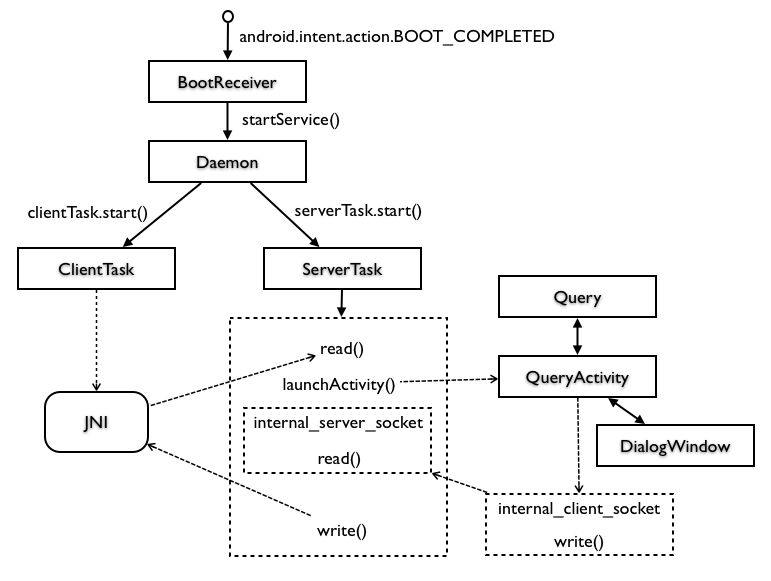
\includegraphics[scale=0.5]{figures/dg_java_flow.png}
 \caption{Process flow in the Java layer}
 \label{fig:dg_java_flow}
\end{figure}

The process flow of the Java layer is illustrated in \autoref{fig:dg_java_flow}. It presents the following classes:

\begin{itemize}
\item \texttt{BootReceiver}: operates as a \textit{BroadcastReceiver} that starts DroidGuardian after the device booting process.
\item \texttt{Daemon}: acts as a \textit{Service} to run in background while the device is on.
\item \texttt{QueryActivity}: is the \textit{Activity} responsible for displaying the data of queries to the user.
\item \texttt{Query}: does not extend an Android component, being used to translate a native query into a Java query.
\item \texttt{DialogWindow}: is bounded to the \texttt{QueryActivity}, building a fragment to display the dialog window.
\end{itemize}

DroidGuardian was design to run as a daemon, silently and unnoticed, until internet connection requests arose to trigger the dialog window.  Also, applications may launch internet requests at any time since the device starts running. Therefore, DroidGuardian needs to start listening as soon as possible. Android fires an intent immediately after the booting process, allowing applications to receive it:

\indent \texttt{android.intent.action.BOOT\_COMPLETED}

This intent is received trough \textit{Receivers} or \textit{BroadcastReceivers} that overwrite a callback named \texttt{onReceive()}. This method is responsible for grabbing intents and triggering whatever action the developer wants. In this case, the \texttt{BootReceiver}'s \texttt{onReceive()} method starts the daemon allowing DroidGuardian to connect to the kernel module and start listening internet requests.

The following steps describe the process flow of the Java layer:

\begin{enumerate}
\item Android sends \texttt{BOOT\_COMPLETED} intent action and \texttt{BootReceiver} grabs it.
\item \texttt{BootReceiver} starts the service \texttt{Daemon} after grabbing the intent.
\item The \texttt{Daemon} service launches two threads: \texttt{ServerTask} and \texttt{ClientTask}. The former operates as a server in the stream socket protocol and will run until an external perturbation, as low memory, destroys the service. If nothing happen, this socket server will run while the device is on. The last acts as the client socket in this connection. However, the client code is not implemented in this class but in the native library. This thread calls the native method \texttt{startDaemon()} that kicks off the native engine.
\item Once executing, the server socket starts a \texttt{while(1)} loop in which queries' data will be exchanged between the server and the client.
\item When the client gets a query sends it to the server, that receives it through the \etxttt{read()} method of the \texttt{InputStream} interface.
\item Immediately after reading the query, the server invokes an instance of the \texttt{QueryActivity} class through intents, transmitting the query's data.
\item Along with this call to \texttt{QueryActivity}, the server also initializes a new server socket, called internal server, that will handle the communication between the \texttt{Daemon} and the \texttt{QueryActivity}.
\item The \texttt{QueryActivity} gets the query's data in a special format. Then, creates an instance of the \texttt{Query} class, which has as instance variables the fields that will ultimately display the information to the user.
\item This process culminates with the execution of the \texttt{DialogWindow}. The \texttt{QueryActivity} instantiates a new Activity Fragment and exhibits it through the \texttt{show()} method.
\item The \texttt{DialogWindow} fills itself with a View that contains a text, a spinner and buttons. The text displays the internet connection request information so that the user may decide what option to chose in the spinner and what button to click on.
\item Once the user clicks a button, the \texttt{DialogWindow} executes a method that provides from a Java Interface and is implemented in the \texttt{QueryActivity} class. This method starts the internal client socket that will send the user's action to the internal server, listening on the \texttt{Daemon}'s server loop. After sending the message, the internal client closes itself.
\item The internal server gets the information, stores it in a variable and closes itself.
\item At last, the server reads this variable's value and sends the message back to the native client.
\item This process is repeated every time a new connection request reaches the Java layer.
\end{enumerate} 

\section{Decisions}

While developing DroidGuardian, various doubts and questions came out regarding the best way to implement certain features. This section presents those cases along with the decision taken and its explanation.

\subsubsection{Dialog vs Notification}

The dialog window don't follow the correct rules that Android states when it comes to alert the user that some event occurred. Dialogs exist for this purpose, but in a different context. A dialog alert should be used inside an activity that the user intentionally invoked. For instance, when the user triggers an action to delete data from a certain folder it is expected that a dialog window pops up asking if he intends to delete that data. This is a consequence of the user's action.

In situations where an event occurs outside the application that the user is interacting with, Android offers the \textit{Notification} interface. Notifications are messages displayed on the notification bar, placed at the top (or bottom) of Android devices, by icons. When a new icon appears on the notification bar, it means that some event took place as a result from a background action. The user is able to expand the notification bar to check all notifications that, usually, comprise some short information text. By clicking on the notification area, it may fill the screen with data related to the event that occurred, depending on how the notification was developed. Users are free to keep notifications unread for as long as they want, without lose performance.

Considering both elements, dialogs and notification, the DroidGuardian case fits better in the last, because the event that triggers an alert to the user happens in background. However, taking the internet connection request to the notification bar would lead to a longest response time when compared to the dialog. The time the user takes to provide his input is included in the total amount of time that the socket waits in the kernel in order to accept or reject the connection. It is known that kernel operations should be executed as fast as possible and that keeping the kernel stuck could bring several damages to the system. Even though it is kept waiting a considerable amount of time using dialogs, compared to notifications this time would increase. 

It was decided that disrupt the user from whatever he is doing, with an alert pop up was better than keeping the kernel waiting long periods of time.

\subsubsection{Service and Activity communication}

The communication between the \texttt{Daemon} and the \texttt{QueryActivity} is established through local sockets. This is the third nested socket connection that takes place since DroidGuardian intercepts an internet connection attempt in the kernel and displays it to the user.

